\documentclass{beamer}
% Naloga 1.3.1: Za dokument uporabite razred `beamer'.

% Ne dodajajte nastavitve za velikost pisave, kot je bila v datoteki `5-prosojnice.tex`.

% Naloga 1.3.2: vključite paket `predavanja'.
\usepackage{predavanja}

% Naloga 1.3.3: definirajte okolje `izrek'.
\usepackage{amsmath}
\usepackage{amssymb}
\newtheorem{izrek}{Izrek}
% Namig: z iskanjem po datotekah (Ctrl+Shift+F oz. Cmd+Shift+F) 
% poiščite niz `{izrek}'.

\usepackage{array}
\usepackage{tikz}
\usetikzlibrary{intersections}



\begin{document}
\title{Matematični izrazi in uporaba paketa \texttt{beamer}}
% - naslov: Matematični izrazi in uporaba paketa \texttt{beamer}
  \subtitle{Vaje pri predmetu \emph{Računalniški praktikum}}
% - podnaslov: Vaje pri predmetu \emph{Računalniški praktikum}
  \institute{Fakulteta za matematiko in fiziko}
% - ustanova: Fakulteta za matematiko in fiziko
  \date{}
% - datum: naj se ne izpiše; to dosežete z ukazom \date{}.

\begin{frame}
 \titlepage
    
\end{frame}

% Zgornje podatke nastavite z ukazi kot v dokumentih razreda `article`.
% Več o tem, kako se naredi naslovno stran, si preberite na naslovu:
% https://www.overleaf.com/learn/latex/Beamer
% To stran preberite do vključno razdelka "Creating a table of contents".
% Ukaz `\titlepage` deluje podobno kot ukaz `\maketitle`, ki ste ga že srečali.



% Naloga 1.3.5: pripravite kazalo vsebine.
\begin{frame}
  \frametitle{Kratek pregled} %[pausesections]
  \tableofcontents
    
\end{frame}
% 1. Naslov prosojnice s kazalom vsebine naj bo "Kratek pregled".
% 2. Z neobveznim argumentom `pausesections' (v oglatih oklepajih)
%    določite, da se kazalo vsebine odkriva postopoma.
%    Poglejte, kako deluje ta ukaz.
% 3. Ker ni videti preveč lepo, neobvezni argument zakomentirajte.

\section{Paket \texttt{beamer}}
% Naslov prosojnice lahko napišemo tudi kot argument okolja `frame`.
\begin{frame}{Posebnosti prosojnic}
	% Naloga 2.3.1:
	% Dodajte ukaze, ki bodo poskrbeli, da se bo prosojnica odkrivala postopoma,
	% tako kot v datoteki prosojnice-resitev.pdf

	Za prosojnice je značilna uporaba okolja \texttt{frame},
	s katerim definiramo posamezno prosojnico,
	\pause
	postopno odkrivanje prosojnic,
	\pause
	ter nekateri drugi ukazi, ki jih najdemo v paketu \texttt{beamer}.
	\pause
	\begin{exampleblock}{Primer}
		Verjetno ste že opazili, da za naslovno prosojnico niste uporabili
		ukaza \texttt{maketitle}, ampak ukaz \texttt{titlepage}.
	\end{exampleblock}
\end{frame}

\begin{frame}{Poudarjeni bloki}
	% Naloga 2.3.2:
	% Oblikujte poudarjena bloka z opombo in opozorilom.

\begin{block}{Opomba}
	Okolja za poudarjene bloke so \texttt{block}, \texttt{exampleblock} in \texttt{alertblock}.
\end{block}

\begin{block}{\alert{Pozor!}}
	Začetek poudarjenega bloka (ukaz \texttt{begin}) vedno sprejme 
		dva argumenta: okolje in naslov bloka.
		Drugi argument (za naslov) je lahko prazen. 
\end{block}

		

\end{frame}

\begin{frame}{Tudi v predstavitvah lahko pišemo izreke in dokaze}
	% Naloga 2.3.3:
	% Oblikujte okolje itemize, tako da se bo njegova vsebina postopoma odkrivala.
	% Ne smete uporabiti ukaza `pause'.
	% Beseda `največje' naj bo poudarjena šele na četrti podprosojnici.

	\begin{izrek}
	   Praštevil je neskončno mnogo.
	\end{izrek}
	\begin{proof}
	   Denimo, da je praštevil končno mnogo.
		% Z neobveznim argumentom [<+->] okolja itemize določimo,
		% da se elementi naštevanja odkrivajo postopoma.
	   \begin{itemize}[<+->]
		  \item Naj bo \(p\) \alert<4>{največje} praštevilo.
		  \item Naj bo \(q\) produkt števil \(1\), \(2\), \ldots, \(p\).
		  \item Število \(q+1\) ni deljivo z nobenim praštevilom, torej je \(q+1\) praštevilo.
		  \item To je protislovje, saj je \(q+1>p\). \qedhere
	   \end{itemize}
	\end{proof}
 \end{frame}
 


\section{Paketa \texttt{amsmath} in \texttt{amsfonts}}
\begin{frame}{Postopno odkrivanje v okolju align}
	% Naloga 3.2:
	% Za pravilno postopno odkrivanje morate na enem mestu uporabiti ukaz `only',
	% na dveh pa ukaz `onslide'.
	% Namig: prva vrstica enačbe se od druge podprosojnice naprej nadaljuje
	% z vsebino druge vrstice. To dosežete tako, da z ukazom `only' samo na prvi
	% podprosojnici postavite del prve vrstice od znaka & do znakov \\,
	% vključno z njimi:
	%     (a+b)^n \only<1>{&= \ldots \\}
	% Na poznejših podprosojnicah tako ni ne treh pik ne konca vrstice,
	% zato se za (a+b)^n izpiše naslednja vrstica.
	Dokaži \emph{binomsko formulo}: za vsaki realni števili \(a\) in \(b\) in za vsako naravno število \(n\) velja
	\begin{align*}
	(a+b)^n \only<1>{&= \ldots \\}
    \onslide<2-3>{&= (a+b) (a+b) \dots (a+b) \\}
	\onslide<3>{&= a^n + n a^{n-1} b + \dots + \binom{n}{k} a^{n-k} b^k + \dots + n a b^{n-1} + b^n \\}
	&= \sum_{k=0}^n \binom{n}{k} a^{n-k} b^k
	\end{align*}
\end{frame}


\section{Stolpci in slike}
\begin{frame}{Konstrukcija pravokotnice}

	
 \begin{columns}
		
	
  \begin{column}{0.55\textwidth}
    \begin{itemize}[<+->]
		\item Dana sta premica \(p\) in točka \(T\).
		\item Nariši lok \(k\) s središčem v \(T\).
		\item Lok \(k\) seče premico \(p\) v točkah \(A\) in \(B\).
		\item Nariši lok \(m\) s središčem v \(A\).
		\item Nariši lok \(n\) s središčem v \(B\) in z enakim polmerom.
		\item Loka se sečeta v točki \(C\).
		\item Premica \(TC\) je pravokotna na \(p\).
	\end{itemize}
  \end{column}

  \begin{column}{0.45\textwidth}
    \centering
    \includegraphics<1>[width=50mm]{slike/fig-1.png}%
	\includegraphics<2>[width=50mm]{slike/fig-2.png}%
    \includegraphics<3>[width=50mm]{slike/fig-3.png}%
	\includegraphics<4>[width=50mm]{slike/fig-4.png}%
	\includegraphics<5>[width=50mm]{slike/fig-5.png}%
    \includegraphics<6>[width=50mm]{slike/fig-6.png}%
    \includegraphics<7>[width=50mm]{slike/fig-7.png}%
  \end{column}
 \end{columns}

   
\end{frame}

  

\section{Paket \texttt{beamer} in tabele}
\begin{frame}{Odkrivanje tabele po vrsticah}
	Včasih pride prav, da tabelo odkrivamo postopoma po vrsticah.
	\begin{center}
		\begin{tabular}{c|cccc}
		   Oznaka & A & B & C & D \\ \hline
		   \pause
		   X & 1 & 2 & 3 & 4 \\
           \pause
		   Y & 3 & 4 & 5 & 6 \\
           \pause
		   Z & 5 & 6 & 7 & 8
		\end{tabular}
	\end{center}
\end{frame}
 

\begin{frame}{Odkrivanje tabele po stolpcih}
	Tabelo lahko odkrivamo tudi po stolpcih, čeprav ni najlažje.

	\begin{center}
		\begin{tabular}{c|>{\onslide<2->}c>{\onslide<3->}c>{\onslide<4->}c>{\onslide<5->}c<{\onslide}}
		   Oznaka & A & B & C & D \\ \hline
		   X & 1 & 2 & 3 & 4 \\
		   Y & 3 & 4 & 5 & 6 \\
		   Z & 5 & 6 & 7 & 8
		\end{tabular}
	\end{center}
\end{frame}


\section{Risanje s paketom TikZ}
\begin{frame}{Konstrukcija pravokotnice}
	\centering
	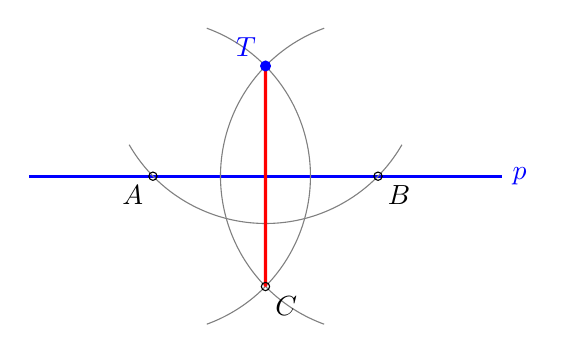
\begin{tikzpicture}
		\coordinate (T) at (0, 1.4);
		\draw[blue, very thick, name path=p] (-3, 0) -- (3, 0) node[right] {$p$};
		\pause
		\draw[gray, name path=k] (T) ++(210:2) arc (210:330:2);
		\path[name intersections={of=p and k, by={A, B}}];
		\pause
		\draw[gray, name path=m] (A) ++(-70:2) arc (-70:70:2);
		\pause
		\draw[gray, name path=n] (B) ++(250:2) arc (250:110:2);
		\pause
		\path[name intersections={of=m and n, by={C, T'}}];
		\pause
		\draw[red, very thick] (T) -- (C);
		\onslide\fill[blue] (T) circle (2pt) node[above left] {$T$};
		\onslide<2->\draw (A) circle (1.5pt) node[below left] {$A$};
		        \draw (B) circle (1.5pt) node[below right] {$B$};
		\onslide<5->\draw (C) circle (1.5pt) node[below right] {$C$};
	\end{tikzpicture}
\end{frame}


\end{document}